\documentclass{ppgeesa}

\usepackage[hidelinks]{hyperref}
\usepackage{url}
\usepackage{breakurl}

\usepackage[detect-weight,detect-family]{siunitx}
\sisetup{output-decimal-marker = {,}}
\sisetup{exponent-product = {\cdot}}

\usepackage{Math}
\mathtoolsset{showonlyrefs}
\usepackage{resizegather}
\usepackage{icomma}
\renewcommand{\Prod}{\,}

\usepackage{Figure}
\graphicspath{{../img/}}

\usepackage[inline]{enumitem}

% siunitx % cspell:disable-line
\DeclareSIUnit{\med}{med}
\DeclareSIUnit{\day}{dia}

\hyphenation{ARX ARMAX OE BJ}

\begin{document}
\bstctlcite{IEEEBST:Brazilian}

\title{Identificação de Sistema Linear por Erro de Predição}
\author{Guilherme de Paoli Beal
  \\
  {\small Universidade Federal do Rio Grande do Sul}
  \thanks{G. Beal, guilherme.beal@ufrgs.br}
}
\maketitle
\thispagestyle{empty}\pagestyle{empty}

\begin{abstract}
  Aqui vai o resumo.
\end{abstract}

\begin{IEEEkeywords}
  Identificação, Sistema Linear
\end{IEEEkeywords}

\section{Introdução}

%% TODO desenvolver introdução

As implementações são desenvolvidas em Python, versão 3.9.12.
A identificação por erro de predição utiliza o pacote \texttt{pysid} em versão de desenvolvimento 0.1.0.
O código deste projeto está publicado em \href{https://github.com/GuiBeal/system-identification}{\texttt{github.com/GuiBeal/system-identification}}.

\section{Identificação por Erro de Predição}

Considere um sistema discreto, linear, invariante no tempo, com uma única entrada e uma única saída.
A resposta deste sistema é dada por
\begin{equation}\label{eq:system}
  y(t) = G_0(z) \Prod u(t) + \nu(t)
  ,\; t \in \mathbb{N}
  ,
\end{equation}
em que
$y(t)$ é o sinal de saída,
$G_0(z)$ é a função de transferência do sistema,
$u(t)$ é o sinal de entrada,
$\nu(t)$ é um ruído de medição desconhecido, %% TODO verificar nomenclatura
$z$ é o operador de avanço --- de modo que $z \Prod x(t) = x(t+1)$ --- e
$t \in \mathbb{N}$ é a variável de tempo discreto.

\subsection{Modelos}

O modelo busca representar o sistema real $G_0(q)$ expresso em \eqref{eq:system}.
Em particular, na identificação por erro de predição, o modelo procurar caracterizar também o ruído $\nu(t)$.

Quatro diferentes classes de modelo são exploradas neste trabalho:
\begin{itemize}
  \item Autorregressivo com Entrada Externa, ou \textit{Autoregressive with Extra Input} (ARX);
  \item Autorregressivo com Média Móvel e Entrada Externa, ou \textit{Autoregressive Moving Average with Extra Input} (ARMAX);
  \item Erro na Saída, ou \textit{Output Error} (OE); e
  \item Box-Jenkins (BJ).
\end{itemize}
Essas classes são casos particulares de um modelo mais genérico, definido por
\begin{equation}\label{eq:model}
  A(q) \Prod y(t) = \dfrac{B(q)}{F(q)} \Prod u(t) + \dfrac{C(q)}{D(q)} \Prod e(t)
  ,
\end{equation}
em que $e(t)$ é ruído branco.
Os polinômios têm os formatos
\begin{align}
  A(q) &= 1 + a_1 \Prod q^{-1} + \dotsb + a_{n_a} \Prod q^{-n_a}
  ,
  \\
  B(q) &= q^{-n_k} \Prod \left(b_0 + b_1 \Prod q^{-1} + \dotsb + b_{n_b} \Prod q^{-n_b}\right)
  ,
  \\
  C(q) &= 1 + c_1 \Prod q^{-1} + \dotsb + c_{n_c} \Prod q^{-n_c}
  ,
  \\
  D(q) &= 1 + d_1 \Prod q^{-1} + \dotsb + d_{n_d} \Prod q^{-n_d}
  , \text{ e}
  \\
  F(q) &= 1 + f_1 \Prod q^{-1} + \dotsb + f_{n_f} \Prod q^{-n_f}
  ,
\end{align}
em que $n_a$, $n_b$, $n_c$, $n_d$ e $n_f$ são as ordens dos polinômios e $n_k$ é o número de atrasos da entrada para a saída.
Definindo as funções de transferência
\begin{align}
  G(q) &= \dfrac{B(q)}{A(q) \Prod F(q)}
  , \text{ e}
  \\
  H(q) &= \dfrac{C(q)}{A(q) \Prod D(q)}
  ,
\end{align}
então \eqref{eq:model} pode ser reescrita como
\begin{equation}\label{eq:model-tf}
  y(t) = G(q) \Prod u(t) + H(q) \Prod e(t)
  .
\end{equation}
Note que $G(q)$ caracteriza o sistema real $G_0(q)$.
Por sua vez, o ruído de medição $\nu(t)$ é representado como ruído branco $e(t)$ filtrado por $H(q)$: %% TODO revisar nomenclatura
\begin{equation}
  \nu(t) = H(q) \Prod e(t)
  .
\end{equation}

Pelas definições dos polinômios,
\begin{equation}\label{eq:H-inf}
  H(\infty) = 1
  .
\end{equation}
Outrossim, se o modelo representa um sistema amostrado, então $G(q)$ deve ser estritamente própria --- isto é, o grau de seu denominador é maior que o de seu numerador --- o que é garantido com $n_k \geq 1$.

Ressalta-se que este modelo genérico pode apresentar definições e notações diferentes, como em \cite{book:Ljung1999, book:Aguirre2007, misc:matlab-polynomial-models}.
A definição aqui apresentada corresponde aos formatos dos polinômios retornados pelas funções do pacote \texttt{pysid}.

\subsection{Predição}

A predição é realizada aplicando
\begin{equation}\label{eq:prediction}
  \hat{y}(t) = L_u(q) \Prod u(t) + L_y(q) \Prod y(t)
\end{equation}
com
\begin{align}
  L_u(q) &= \dfrac{G(q)}{H(q)}
  , \text{ e}
  \\
  L_y(q) &= 1 - \dfrac{1}{H(q)}
  .
\end{align}
Embora isso não seja diretamente evidenciado por \eqref{eq:prediction}, o fato de $G(q)$ ser estritamente própria juntamente com \eqref{eq:H-inf} garante que a predição $\hat{y}(t)$ no instante $t = t_0$ depende somente de valores de $u(t)$ e $y(t)$ em instantes $t < t_0$ --- isto é, a predição é realizado a partir de valores anteriores dos sinais de entrada e saída medidos.

O erro de predição é definido como
\begin{equation}
  \varepsilon(t)
  = y(t) - \hat{y}(t)
  = \dfrac{y(t) - G(q) \Prod u(t)}{H(q)}
  .
\end{equation}
Assim, o erro quadrático médio de predição é definido por
\begin{equation}\label{eq:mse}
  J = \dfrac{1}{N} \Prod \Sum{t=1}{N}{\Round{\varepsilon(t)}^2}
  .
\end{equation}

\subsection{Identificação}
A identificação por erro de predição visa, a partir de um conjunto de dados de entrada $u(t)$ e de saída $y(t)$ medidos do processo, a identificar os parâmetros dos polinômios do modelo de forma a minimizar o custo expresso em \eqref{eq:mse}.
O algoritmo aplicado neste processo depende da classe do modelo e está fora do escopo deste trabalho.
Estes são implementados pelo pacote \texttt{pysid}.

\subsection{Classes de Modelos}

\subsubsection{ARX}
No modelo ARX há liberdade nas escolhas de $n_a$, $n_b$ e $n_k$, enquanto $n_c = n_d = n_f = 0$.
Assim, as funções de transferência tornam-se
\begin{align}
  G(q) &= \dfrac{B(q)}{A(q)}
  , \text{ e}
  \\
  H(q) &= \dfrac{1}{A(q)}
  .
\end{align}
Esta classe tem a vantagem de resultar numa minimização linear nos parâmetros, os quais podem ser obtidos por mínimos quadrados.

\subsubsection{ARMAX}
O modelo ARMAX requer a arbitração das ordens $n_a$, $n_b$, $n_c$ e $n_k$, com $n_d = n_f = 0$.
Portanto, as funções de transferência são
\begin{align}
  G(q) &= \dfrac{B(q)}{A(q)}
  , \text{ e}
  \\
  H(q) &= \dfrac{C(q)}{A(q)}
  .
\end{align}

\subsubsection{\emph{Output Error}}
Para o modelo OE são escolhidas as ordens $n_b$, $n_f$ e $n_k$, fixando $n_a = n_c = n_d = 0$.
Nesse casso, tem-se
\begin{align}
  G(q) &= \dfrac{B(q)}{F(q)}
  , \text{ e}
  \\
  H(q) &= 1
  .
\end{align}
Note que este modelo considera que o ruído de medição é ruído branco. % TODO nomenclatura

\subsubsection{Box-Jenkins}
Finalmente, no modelo BJ arbitra-se $n_b$, $n_c$, $n_d$, $n_f$ e $n_k$, com $n_a = 0$.
Com isso, obtém-se
\begin{align}
  G(q) &= \dfrac{B(q)}{F(q)}
  , \text{ e}
  \\
  H(q) &= \dfrac{C(q)}{F(q)}
  .
\end{align}

\section{Dados}

Os dados são apresentados na Figura \ref{fig:data}, em que o sinal $u(t)$ é multiplicado por um fator de $10$ para melhor visualização.
Ambos os sinais $u(t)$ e $y(t)$ contêm 200 amostras.

\begin{figure}[!htbp]
  \centering
  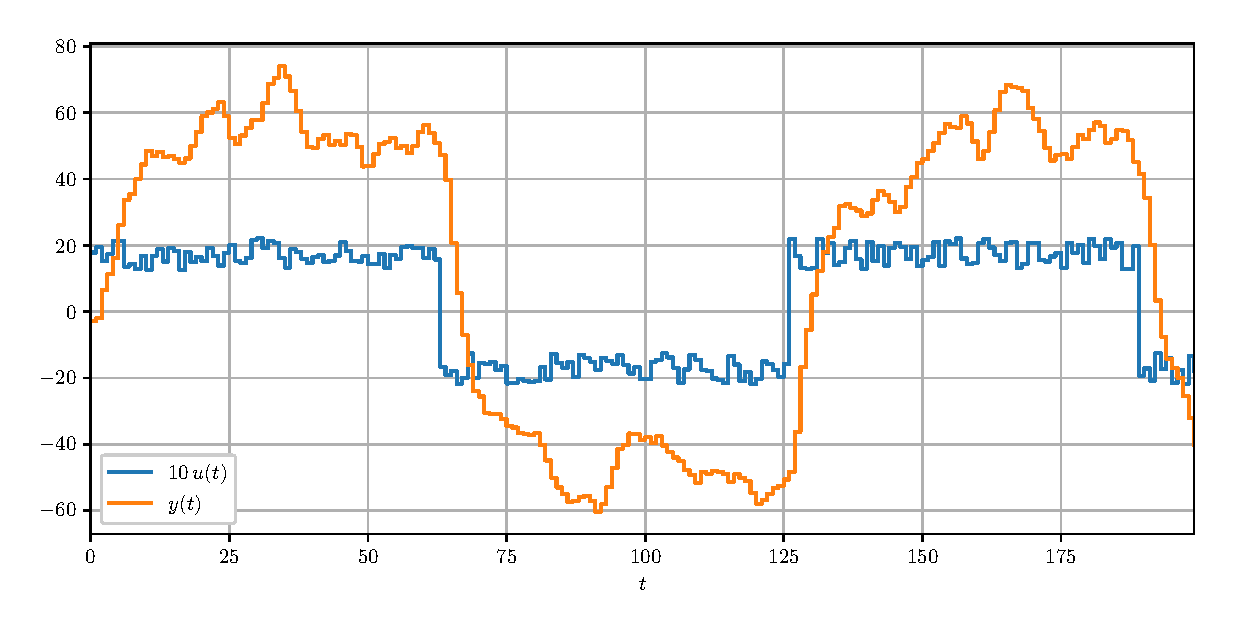
\includegraphics[width=\linewidth]{data}
  \caption{Dados de entrada e saída.}
  \label{fig:data}
\end{figure}

\section{Resultados}

% \subsection{ARX}

% Variando $n_a \in \Set{0, 1, 2, 3}$, $n_b \in \Set{0, 1, 2, 3}$ e $n_k \in \Set{1, 2, 3}$ são obtidos XX modelos ARX.
% A tabela

\begin{table}[!htbp]
  \centering
  \caption{Modelos ARX melhor classificados.}
  \begin{tabular}{|c|c|c|c|}
    \hline
    \# & $n_a$ & $n_b$ & $n_k$ \\\hline\hline
    \\\hline
  \end{tabular}
  \label{tab:arx}
\end{table}
\section{Conclusões}

\bibliographystyle{IEEEtran}
\bibliography{bib/book, bib/misc, bib/controlIEEE}

\end{document}
